\chapter{Effects of Network Topology}

\section{Node Distance from the Anchors}

Of great assistance to network designers is to know in which regions of the network to expect poor localization performance.  With this information, and if the anchor placement is constrained, they could either avoid placing nodes in the expected poor area, or take into account the higher expected localization errors in the analysis of the data.

Figure~\ref{fig:AS6goodcontour} shows a different view of in-network errors. Instead of showing a line representing the localization errors as in other figures present in this study, the error at each node is used to interpolate a grid of location errors throughout the area of the network.  A contour plot, based on that interpolated grid, is then shown in the figure.  The goal in viewing the network map in this way is to discover a pattern in terms of the relationship of a region of the network to the location of the anchor nodes.  Unfortunately, no geographic correlation between location error and anchor node placement can be ascertained.  It may be possible, with future study, to remove the effect of other factors to reveal a pattern based on anchor placement.

\begin{figure}
  \centering
	\subfloat[Network A]{
		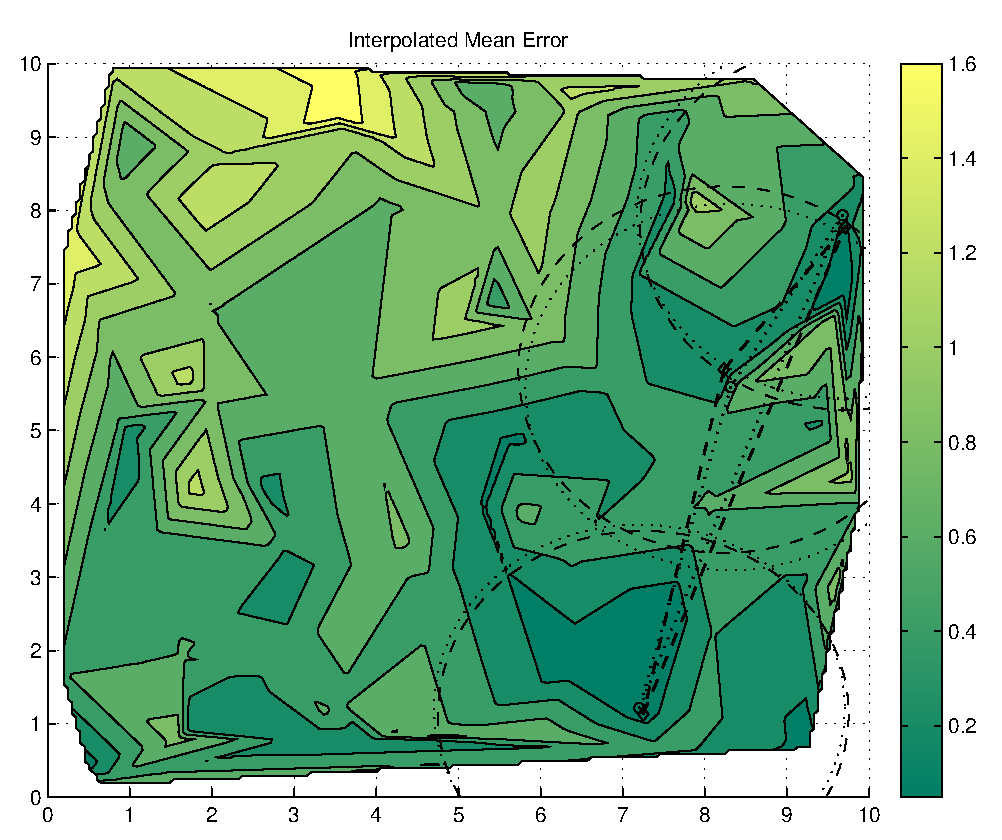
\includegraphics[width=\figurewidth\textwidth]{outliers/AS6/AS6NetworkContour7}}
	\\
	\subfloat[Network B]{
		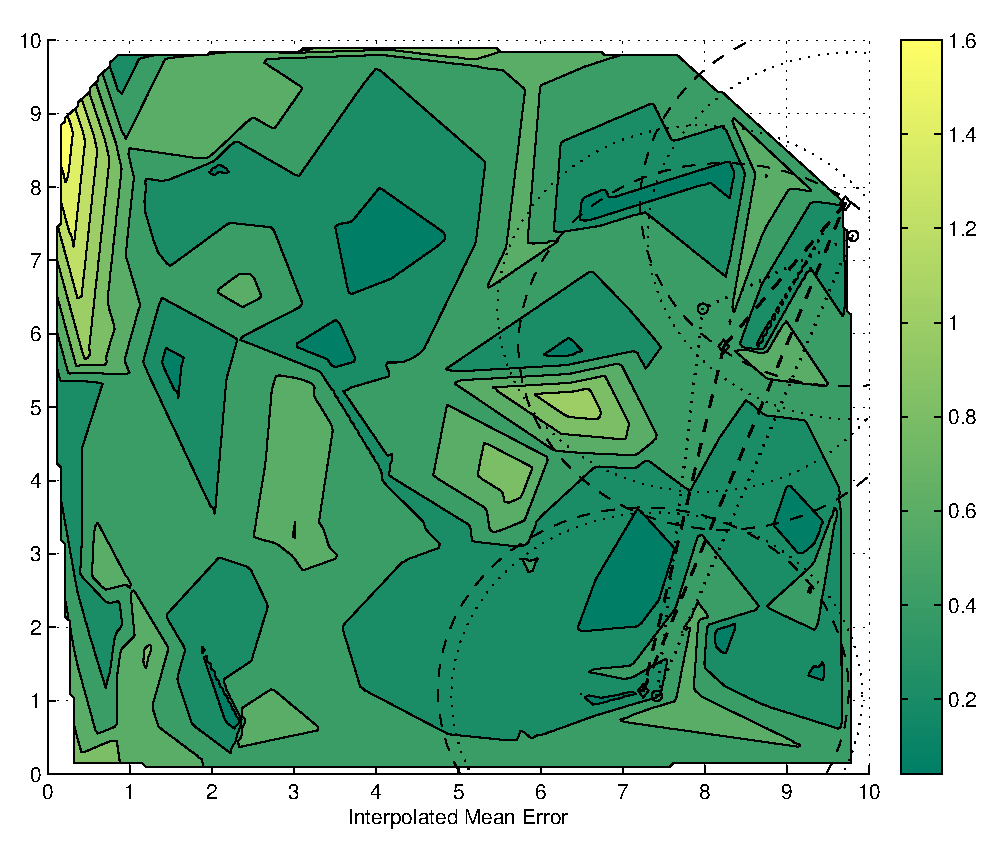
\includegraphics[width=\figurewidth\textwidth]{outliers/AS6/AS6NetworkContour10}}
	\caption{Localization error as a contour plot}
	\label{fig:AS6goodcontour}
\end{figure}

\section{Applicability to Varying Network Topologies}

So far, we have examined anchor node placement for a continuous square network, with randomly placed nodes.  However, in the real world, networks are not alway so simple.  There are often regions in the network where it is not possible to put nodes, due to physical barriers like lake, buildings or access to property.  In this section, we look at how the results thus far apply to C-shaped and long, narrow pipeline network topologies.

\subsection{C-Shape Network Topology}

A C-shape network consists of a relatively square region with an empty area on one side, as shown in Figure~\ref{fig:cnetwork}.  In terms of anchor placement requirements, we do not expect any difference between the recommendations presented for square networks.

\begin{figure}
  \centering
	\includegraphics[width=\textwidth]{cshape/network}
	\caption{Example of C-shape network topology}
	\label{fig:cnetwork}
\end{figure}

To show that there is no difference, 10 random networks with 5000 anchor sets each was simulated in the same manner as the square networks.  Figure~\ref{fig:cindicator} shows the location error relative to the sum of the distances between the anchors, as in Section~\ref{sec:bestanchornode}. 
As expected, the mean location error flattens out as the sum of distances between anchor nodes reaches about 10 times the radio range.  There is a slight increase in the mean location error as compared with the square network, but this has to do with the performance of the CCA algorithm itself in the presence of the empty region of nodes in the network.  The increase in mean location error at the end of the plot, and specifically the increase in the confidence interval, is caused by the small sample size in the random selection of anchor set with a very high distance between nodes. 

\begin{figure}
  \centering
	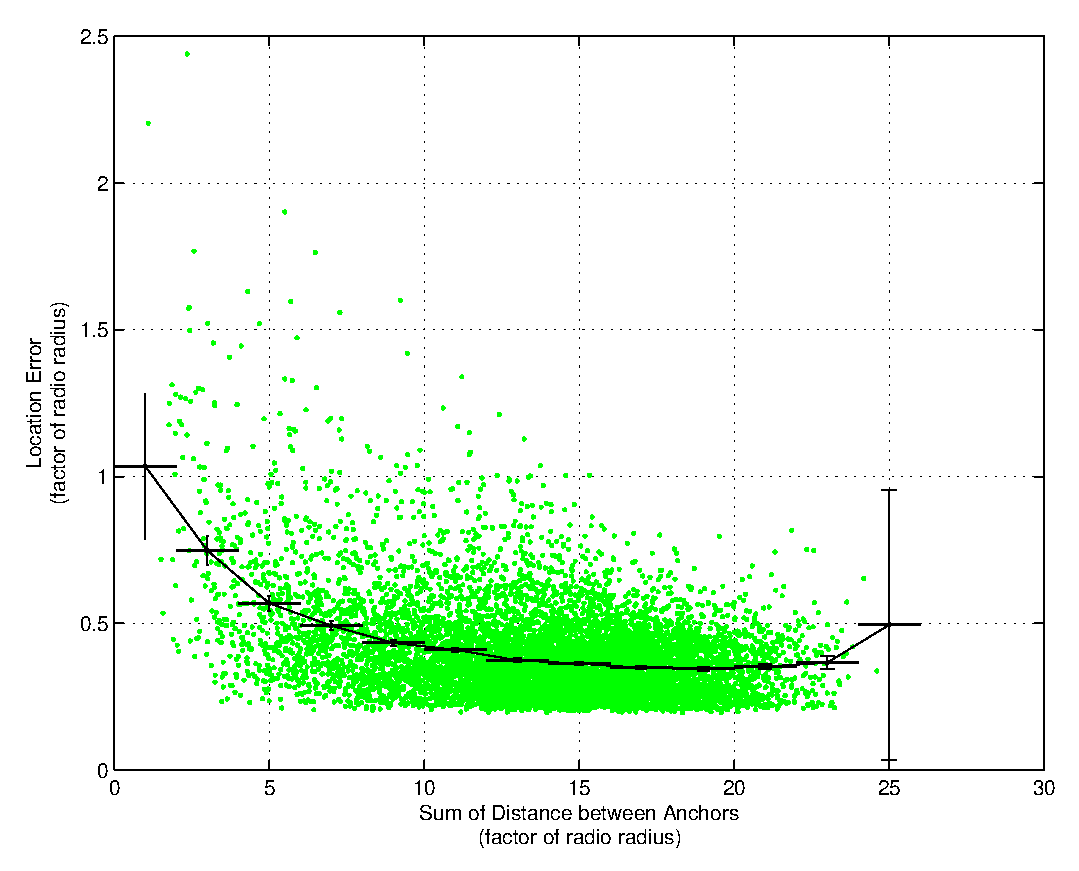
\includegraphics[width=\textwidth]{cshape/SumOfDistanceIndicator_cshape}
	\caption[Sum of distance between anchors vs location error in a C-Shape topology]{Sum of distance between anchors vs location error for 10 random C-shape 20-by-20 unit networks with 400 nodes, 5000 anchor sets each, and a radio range of 2.5 units, excluding outliers}
	\label{fig:cindicator}
\end{figure}

\subsection{Pipeline Network Topology}

In some applications, that network region has very little depth to it, such as gas pipeline or along a highway or railroad line.  The extreme case is where there is a single node placed along a straight axis.  As we have shown, this is the worst possible scenario, as it is the most likely was to cause the outlier condition for localization.  In that case, it is worthwhile to explore the possibility of other localization techniques, such as GPS at each node, or recording the location as the nodes are placed.  

However, for randomly nodes, when there is a bit of depth to the network, as shown in Figure~\ref{fig:pipeline} (not equal x and y scales), there is still the possibility of good localization results.  For pipeline networks with randomly placed nodes, it is much more difficult to meet the network connectivity requirements.  Therefore, the simulations are run for just six networks with 400 nodes in a 200 by 2 unit area.  Note that the width of the pipeline, 2 units, is less than the radio range, 2.5 units.  Also recall that the recommendation to avoid outliers is that the minimum height of the triangle must be a least equal to the radio range, which even the width of the network does not meet. 

Even worse than expected, all of the 30,000 anchor sets across the six networks are outlier cases.  This tells us the the outlier condition in a square network is sometimes avoided by the two-dimensional nature of the square area whereas in a pipeline, the one-dimensional nature is never able to compensate for the collinearity problem.

Figure~\ref{fig:pipelineindicator} shows that that the mean location error is about 20 times the radio range which is well beyond any reasonable value. Interestingly, a relatively small number of anchor sets cause the location error to increase even further when the sum of the distance between anchors is roughly equal to the length of the pipeline.  However, the mean of the mean location error actually dips, although only slightly, while the maximum errors peak.  The peak in maximum mean location errors may be explained by noticing that in order to have a sum of distance between anchors equal to the length of the pipeline, there are two basic scenarios.  First, the three anchor nodes are spread across the entire distance of the network.  This scenario likely falls in the normal range of errors.  The second scenario is when two anchors are roughly collocated, and the third anchor is half the length of the network away.  We suspect that this case causes the worst anchor sets since effectively this is equivalent to having just two anchor nodes.

\begin{figure}
  \centering
	\includegraphics[width=\textwidth]{pipeline/network}
	\caption{Example of pipeline network topology}
	\label{fig:pipeline}
\end{figure}

\begin{figure}
  \centering
	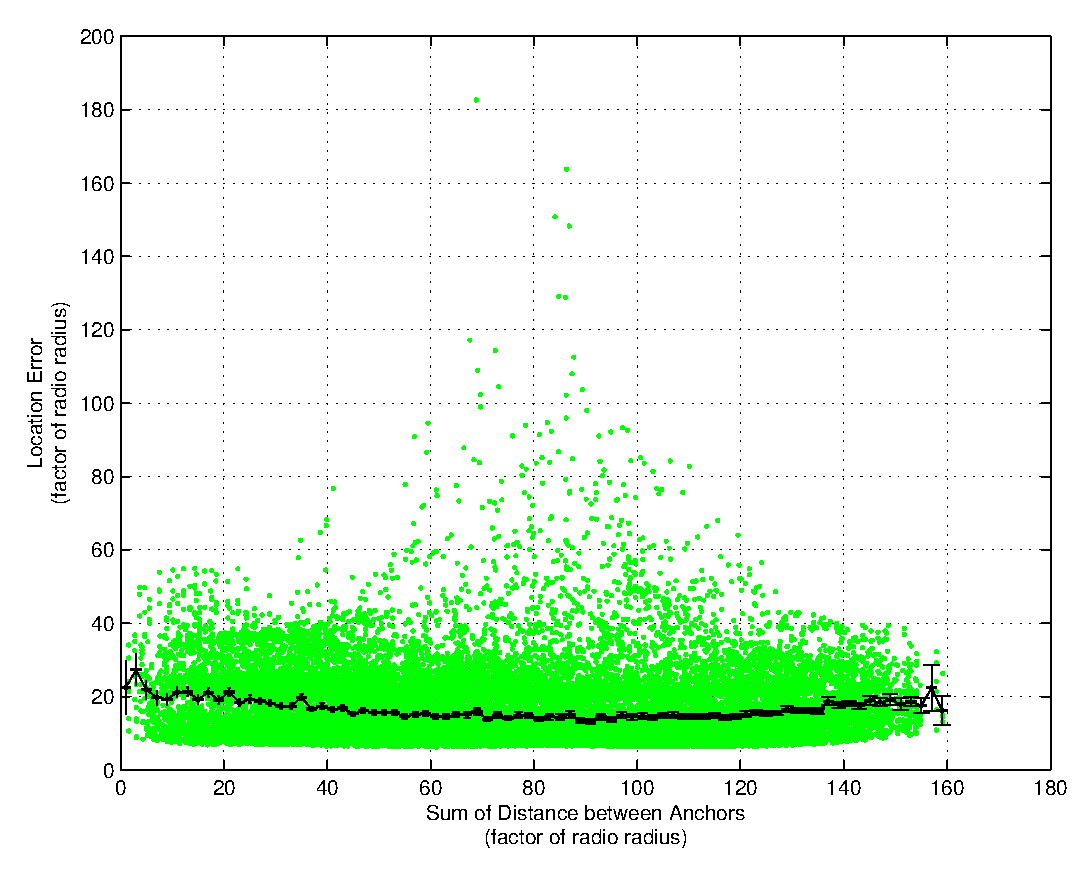
\includegraphics[width=\textwidth]{pipeline/SumOfDistanceIndicator_pipeline}
	\caption[Sum of distances between anchor nodes vs location error in a pipeline topology]{Sum of distances between anchor nodes vs location error for 6 random pipeline 200-by-2 unit networks with 400 nodes, 5000 anchor sets each, and a radio range of 2.5 units}
	\label{fig:pipelineindicator}
\end{figure}

Surprisingly, when the same simulation is run on a 200 by 4 unit area pipeline network where the radio range is 2.5 units, all the anchor sets still provide extremely high location errors.  Figure~\ref{fig:fatpipelineindicator} shows the sum of the distance between anchor nodes versus the mean location error of the network.  The minimum location error in this case is roughly five times the radio range.  However, as compared with the pipeline network where the width of the network is less than the radio range, we now have the inverse relationship between the sum of the distance between anchors and location error in the overall data, but a similar relationship as compared to the mean of the data in both cases.  

The mean location error is lowest when the sum of the distance between anchor nodes is roughly one length of the pipeline.  This can be explained by inferring that when the sum of the distance between anchors is low, the anchors must be clumped together in the pipeline.  In this scenario, only a small portion of the pipeline is covered and therefore leads to poor localization performances. As the sum of the distance between anchors approaches twice the length of the pipeline, two anchors must be at one end of the pipeline and the third anchor at the other end.  Since two of the anchors are therefore more or less collocated, the algorithm again behaves as if there are only two anchor nodes causing poor localization performance.

\begin{figure}
  \centering
	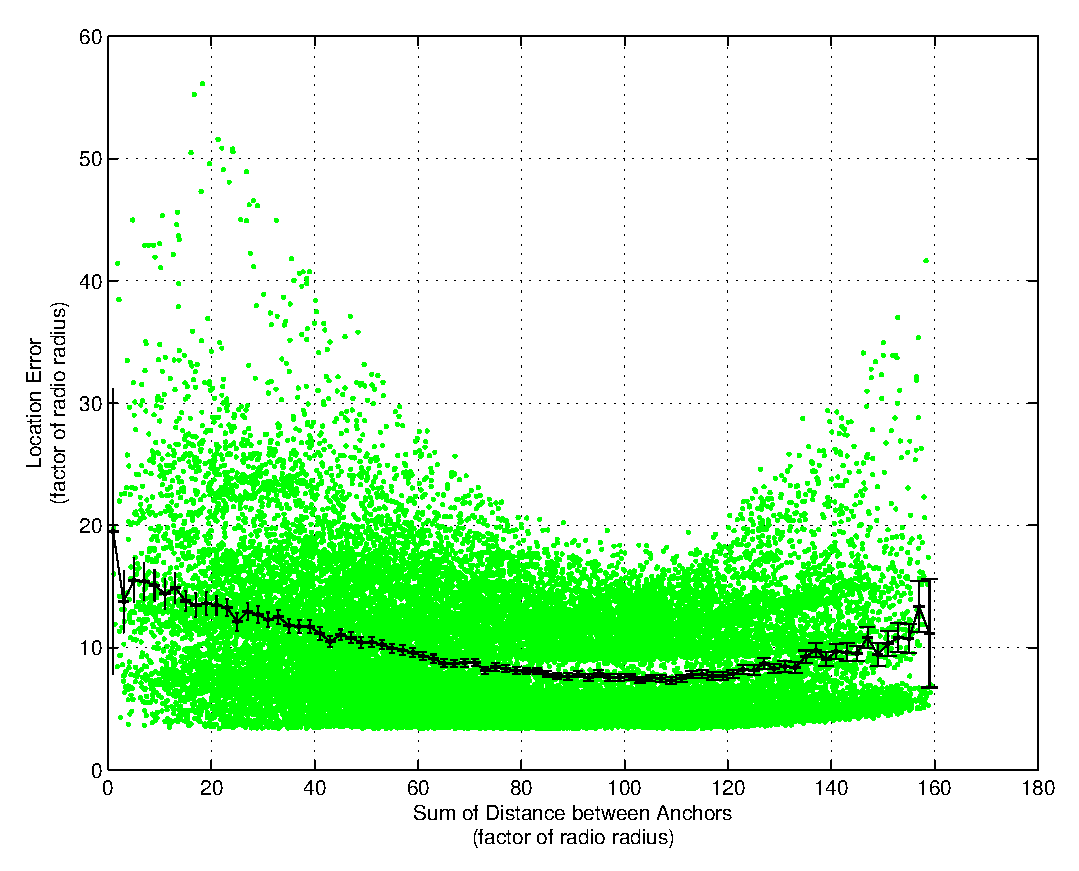
\includegraphics[width=\textwidth]{pipeline/SumOfDistanceIndicator_fatpipeline}
	\caption[Sum of distances between anchor nodes vs location error in a pipeline topology]{Sum of distances between anchor nodes vs location error for 6 random pipeline 200-by-4 unit networks with 800 nodes, 5000 anchor sets each, and a radio range of 2.5 units}
	\label{fig:fatpipelineindicator}
\end{figure}

In the end, even though the results are a bit better when the width of the pipeline is more than the radio range, the localization results are horrible using this method for pipeline network topologies.  Therefore, it is recommended to use a different class of localization algorithms that does not rely on transforming local coordinates into global coordinates with anchor nodes.
